\documentclass[11pt,a4paper]{article}
\usepackage{fullpage}	% Bigger pages
\usepackage{cite} 		% Include citations
\usepackage{hyperref} 	% Hyperlinks everywhere!
\usepackage{natbib}		% Include bibliography
\usepackage{graphicx}	% Include pictures
\usepackage{amsmath}	% Use \eqref

\begin{document}

\title{Constraining the Hemispherical Structure in the Hidden Layer At the Top of the Earth's Inner Core}
\author{Candidate Number: \\  \\ Supervisor: Prof. Keith Priestley}
\maketitle

\begin{abstract}
Since its discovery in 1936, the Earth's inner core has been well documented by both body wave and normal mode studies. However, one area where properties are not yet well measured is the top of the inner core. The upper region of the inner core is of particular interest as it is thought that as the outer core freezes onto the inner core the variable environment at this boundary is encoded in the properties of the frozen material. 
\end{abstract}

\tableofcontents

\newpage
\section{Introduction}
The inner core was first discovered by Inge Lehmann in 1936, who used the existence of P wave arrivals within the P wave shadow zone to infer a solid-liquid boundary lying within the core mantle boundary (\cite{Lehmann}). Over the following 80 years large progress has been made on measuring the properties of the inner core, but there is much still to learn.

Of particular interest is the velocity and attenuation structure, which can be used to infer the chemical and physical properties of the inner core's constituent material. The following gives a summary of these properties, and is quoted directly from \cite{Deuss2014}:
\begin{itemize}
	\item The top 60-80 km of the inner core is isotropic, and the deeper parts have 3-4\% anisotropy. The anisotropy exists in both velocity and attenuation; waves traveling in the polar direction are faster and more attenuated than waves traveling equatorially.
	\item There may be an innermost inner core with different anisotropy, though evidence is not compelling.\footnote{Research published since \cite{Deuss2014} provides strong evidence for this (\cite{Wang2015}).}
	\item The inner core displays a hemispherical variation: The western hemisphere is more strongly anisotropic, has a lower isotropic compressional velocity, and is less attenuating than the eastern hemisphere. There are sharp boundaries between the two hemispheres.
	\item Inner core superrotation is less than $0.5^{\circ}$ /yr and may even be as small as $0.1-1^{\circ}$ /Myr.
\end{itemize}

The upper inner core is of particular interest, as material from the outer core is currently freezing onto it at a rate of around 1mm/year (\cite{Labrosse2001}). Modelling performed by \cite{Deguen2009a} shows that the velocity structure of the upper inner core should reflect recent processes in the lower upper core. Thus measuring the structure of the upper inner core could in turn give insights into areas such as how the outer core generates the Earth's magnetic field. 

So far only large scale velocity structures have been measured, with the most recent velocity models FIND REFERENCES FOR THIS. In addition the extent to which the methodology used here and elsewhere can be applied to the top of the inner core is not well understood. In this paper we tackle both of these problems.

We do so by taking individual earthquakes that travel to multiple seismic stations and identifying the arrival of distinct seismic phases in seismograms. We constrain our analysis to the uppermost inner core as far as is possible, and area not yet investigated in published literature.

Section \ref{sec:Theory} gives an brief theoretical background in seismic body wave theory and inner core sampling, with section \ref{sec:Data} describing our data collection and pre-processing. We then turn to initial analysis of the collected data in \ref{sec:Initial analysis}, after which we take a detour to examine the inherent errors and limits of our methodology in section \ref{sec:Limits}. In the light of section \ref{sec:Limits}, section \ref{sec:Resid measurements} contains a full analysis of our data set and presents updated velocity models for the upper inner core.

%%%
\section{Theoretical Background}
\label{sec:Theory}
In this study we use seismic body wave analysis in order to investigate the velocity structure of the upper inner core. These waves are elastic waves, caused by large earthquakes, that travel from the earthquake source to a receiver station through the interior of the Earth.

\subsection{Body Wave Theory}
Here we summarise the main aspects of seismic body wave theory, taken from \cite{Shearer2009}.

Under the assumptions of a continuous, linearly elastic medium, infinitesimal strains and constant medium properties one can derive the elastic wave equation
\begin{equation}
	\rho \frac{\partial^{2} \vec{u}}{\partial t^{2}} = \left ( \lambda + \mu \right ) \nabla \left ( \nabla \cdot \vec{u} \right ) + \mu \nabla^{2} \vec{u}
	\label{eq:Wave Equation}
\end{equation}
where u is the local displacement vector, $\rho$ the density of the medium and $\lambda$ and $\mu$  Lam\'{e} parameters of the medium. A general displacement vector can be decomposed into irrotational scalar and solenoidal vector potentials such that
\begin{equation}
	\vec{u} \equiv \nabla \phi + \nabla \times \vec{\psi}
	\label{eq:Displacement}
\end{equation}
Substituting \eqref{eq:Displacement} in to \eqref{eq:Wave Equation} yields two independent wave equations, one for $\phi$ and one for $\vec{\psi}$, which describe P-waves and S-waves respectively. P-waves are compressional with displacements occurring parallel to the wave vector, whereas S-waves are transverse with displacements occurring perpendicular to the wave vector. These wave equations take the general form
\begin{equation}
	\frac{\partial^{2} \phi}{\partial t^{2}} = c^{2} \left ( \vec{x} \right ) \nabla^{2} \phi
\end{equation}
$c(\vec{x})$ is the local wave velocity, which depends only on position\footnote{For an anisotropic medium, the wave speed would also depend on the direction of travel of the wave; in this study we assume an isotropic velocity structure throughout.}. A complete velocity model is a full specification of $c(\vec{x})$ in the region of interest.

\subsection{Sampling the Inner Core}
\label{sec:Sampling}
Because the outer core is liquid with $\mu \approx 0$ and thus does not transmit S-waves, it is P-waves that are used to sample the inner core. Figure PUT FIGURE HERE shows the ray path for the PKiKP and PKIKP phase; they travel almost identical paths through the Crust, Mantle and upper Outer Core, after which PKiKP reflects off the Inner Core boundary (ICB), whereas PKIKP travels just underneath the boundary in the Inner Core.

All measurements are compared to the radially symmetric global velocity model from \cite{Kennett1995b} (hereafter called AK135), from which we seek to measure perturbations about. The residual travel time is defined as
\begin{equation}
	\delta t = \left ( t_{PKiKP} - t_{PKIKP} \right )_{observed} -  \left ( t_{PKiKP} - t_{PKIKP} \right )_{model}
	\label{eq:Residual definition}
\end{equation}
where $t$ is the absolute travel time for the phase indicated by the subscript. Observed residuals are those made on real seismograms. Model residuals are those measured on synthetic seismograms, calculated assuming the AK135 model. If we assume that the paths of both the model ray and the real ray are identical, this equation can be reformulated as an integral along the ray paths
\begin{equation}
		\delta t = \left (  \int \frac{1}{v_{obs}} - \frac{1}{v_{model}} ds  \right )_{PKiKP} - \left (  \int \frac{1}{v_{obs}} - \frac{1}{v_{model}} ds \right )_{PKIKP}
		\label{eq:deltat}
\end{equation}
where the path to be integrated along is indicated by the subscript outside the brackets, and in general the velocities can vary as a function of position.

As the inner core has a very low viscosity (eg. \cite{Wijs1998}, \cite{Zhang2000}) we assume that it is unable to sustain any long term non-radial variations in velocity structure. Under this assumption a radially symmetric velocity model is a correct description, so for the outer core $v_{obs} = v_{model}$, setting the first integral in equation \eqref{eq:deltat} to zero.

Taking perturbations about the model of the form $v_{obs} = v_{model} + \delta v$ gives
\begin{equation}
	\delta t =\left ( \int \frac{\delta v}{v_{model} + \delta v }\frac{1}{v_{model}} ds \right )_{PKIKP}
\end{equation}
For depths below the ICB of less than 50km, $v_{model}$ is constant for AK135, and we assume $\delta v$ is also a constant such that we are measuring only the average velocity perturbation along the ray path. Integrating along the model ray path and rearranging, we are thus left with the equation that will allow us to compute $\delta v$
\begin{equation}
	\delta v = \frac{\delta t}{t - \delta t} v_{model}
	\label{eq:Delta v}
\end{equation}
where $t$ is the time PKIKP spends in the inner core in the AK135 model. A positive residual implies a positive velocity perturbation and vice versa, as expected from equation \eqref{eq:Residual definition}.

%%%
\section{Data Selection}
\label{sec:Data}
As discussed in section \ref{sec:Sampling}, we make differential travel time measurements of PKiKP and PKIKP phases. In order to easily measure these phases, an ideal seismogram would have a clear PKIKP arrival, little noise and no interference from surface reflection phases. We measure as many seismograms as possible from each earthquake selected. As such, individual events are selected to meet the following criteria:

\begin{itemize}
	\item Epicentral distance of $115^{\circ}$ - $143^{\circ}$ covers the majority of North America, where there is the highest worldwide density of seismometers.
	\item  Depth greater than 15km, to minimise possible interference between PKIKP (PKiKP) and pPKIKP (pPKiKP) phases\footnote{The preceding 'p' denotes a reflection from the Earth's surface.}.
	\item Magnitude greater than 5.2 and less than 6.3 to ensure a large enough earthquake to produce an observable signal, whilst a small enough earthquake such that the rupture is likely to be impulsive.
	\item A fracture mechanism that is primarily dip slip\footnote{This means a large component of motion is in the vertical direction}. As the ray paths are themselves nearly vertical when they reach the seismic stations (see PUT RAYPATH FIGURE HERE), a significant amount of energy is required to be focused in the vertical direction at the site of the earthquake.
\end{itemize}

Individual earthquakes meeting this criteria typically contain 100 to 600 individual seismograms. Each seismogram is filtered between 0.7Hz - 2Hz in order to focus on the expected frequency of $\sim$1Hz whilst removing unwanted noise at other frequencies. Individual seismograms are then checked by hand, and only those showing a clear PKIKP signal near the predicted arrival time are kept for further analysis. Event parameters are looked up using the Central Moment Tensor (CMT) Catalogue (\cite{Dziewonski1981}, \cite{Ekstrom2012}).

%%%%
\section{Initial data analysis}
\label{sec:Initial analysis}
The same analysis was performed on each individual event. Each event is listed in table \ref{tab:Events}.
\begin{table}\footnotesize
\centering
\begin{tabular}{| l | r | r | c | c | c | c |}
	\hline Location				& Latitude	& Longitude	& Date		& Time		& Magnitude	& Depth (km) 	\\ \hline
	\hline South Sandwich Islands	& -60.13	& -25.38		& 2005/08/04	& 12:11:22	& 5.4			& 34.0		\\
	\hline Mozambique			& -21.27	& 33.57		& 2006/04/14	& 18:41:39	& 5.2			& 30.4		\\
	\hline Uganda				& 1.72	& 30.65		& 2007/02/19	& 02:33:46	& 5.6			& 28.5		\\
	\hline South Sandwich Islands	& -60.04	& -27.46		& 2008/07/30	& 20:15:16	& 5.5			& 145.1		\\
	\hline Tanzania				& -9.50	& 39.22		& 2010/08/03	& 19:42:18	& 5.3			& 32.8		\\
	\hline Banda Sea			& -7.24	& 129.83		& 2013/08/12	& 00:53:45	& 6.1			& 105.2		\\
	\hline Owen Fracture Zone	& 11.35	& 57.43		& 2013/10/02	& 01:06:40	& 5.8			& 19.8		\\
	\hline Celebes Sea			& 4.55	& 122.82		& 2014/04/16	& 04:28:20	& 5.8			& 575.0  		\\ 
	\hline South Sandwich Islands 	& -60.01	& -26.76		& 2014/12/28	& 20:30:58	& 5.2			& 124.4		\\
	\hline N Coast of New Guinea	& -4.51	& 144.00		& 2014/12/31	& 01:37:36	& 5.8			& 133.9		\\
	\hline Tanimbar Islands		& -6.88	& 132.45		& 2015/04/01	& 09:36:01	& 5.5			& 28.6		\\
	\hline	
\end{tabular}
\caption{Event details taken directly from the CMT Catalogue. Dates are formatted as year/month/day format and times as hour:minute:second}
\label{tab:Events}
\end{table}
Here we describe the analysis using data from the Celebes Sea event.

Synthetic waveforms are computed using the WKBJ ray tracing program (\cite{Chapman1976}) combined with rupture mechanisms from the CMT catalogue. Predicted ray paths and individual ray travel times are computed using the TauP toolkit (\cite{Crotwell1999}). Initial plots are shown for both real and synthetic data are shown in the top and bottom of figure \ref{fig:Real nonaligned} respectively, with zero time occurring at the time of the earthquake, taken from the global CMT catalogue. Overplotted are theoretical PKIKP and PKiKP travel times computed using the AK135 model (\cite{Kennett1995b}). The predicted travel times agree well with the data in both cases.  For shorter epicentral distances the predicted arrival times become closer, showing that eventually there will be a phase separation below which the two distinct phases will not be individually observable.

\begin{figure}
	\centering
	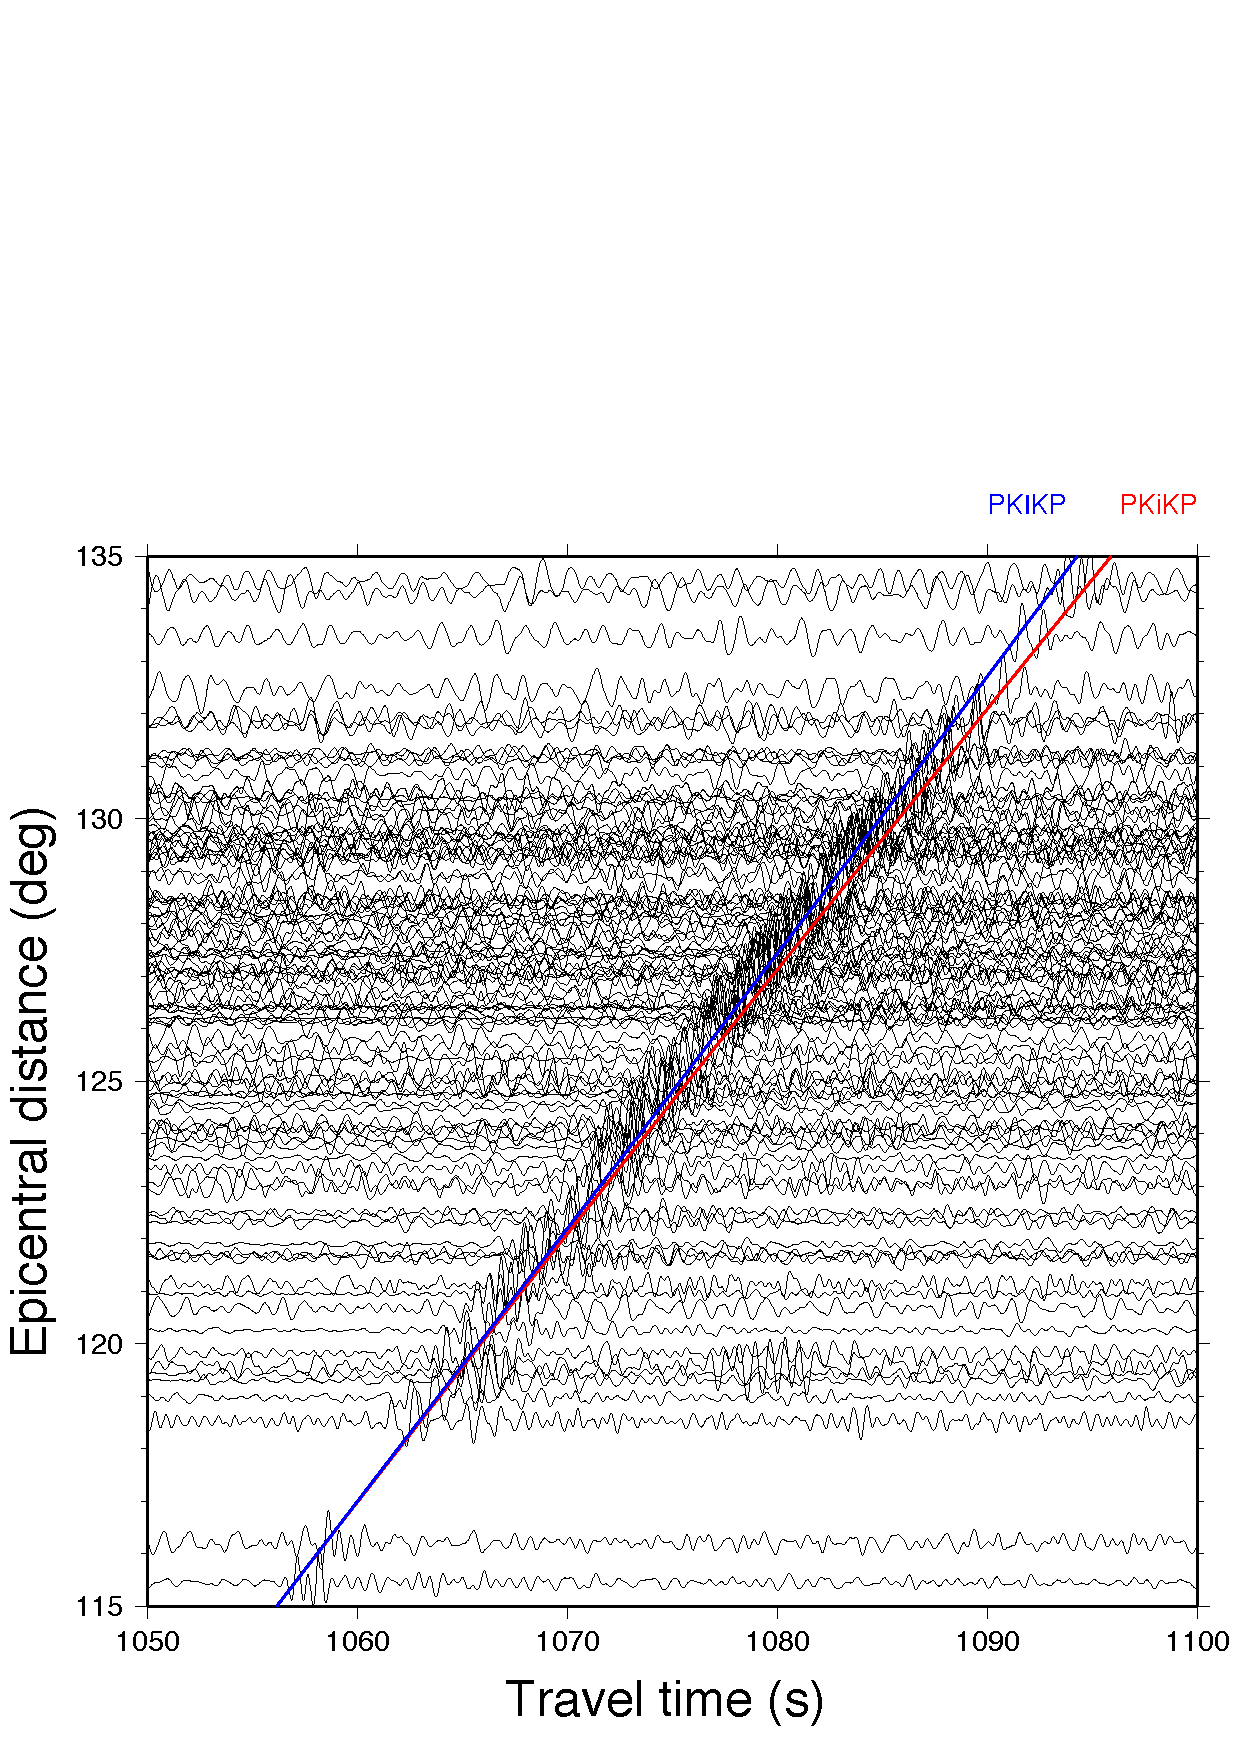
\includegraphics[width=0.6\textwidth]{figures/celebessea/celebessea_real.pdf}
	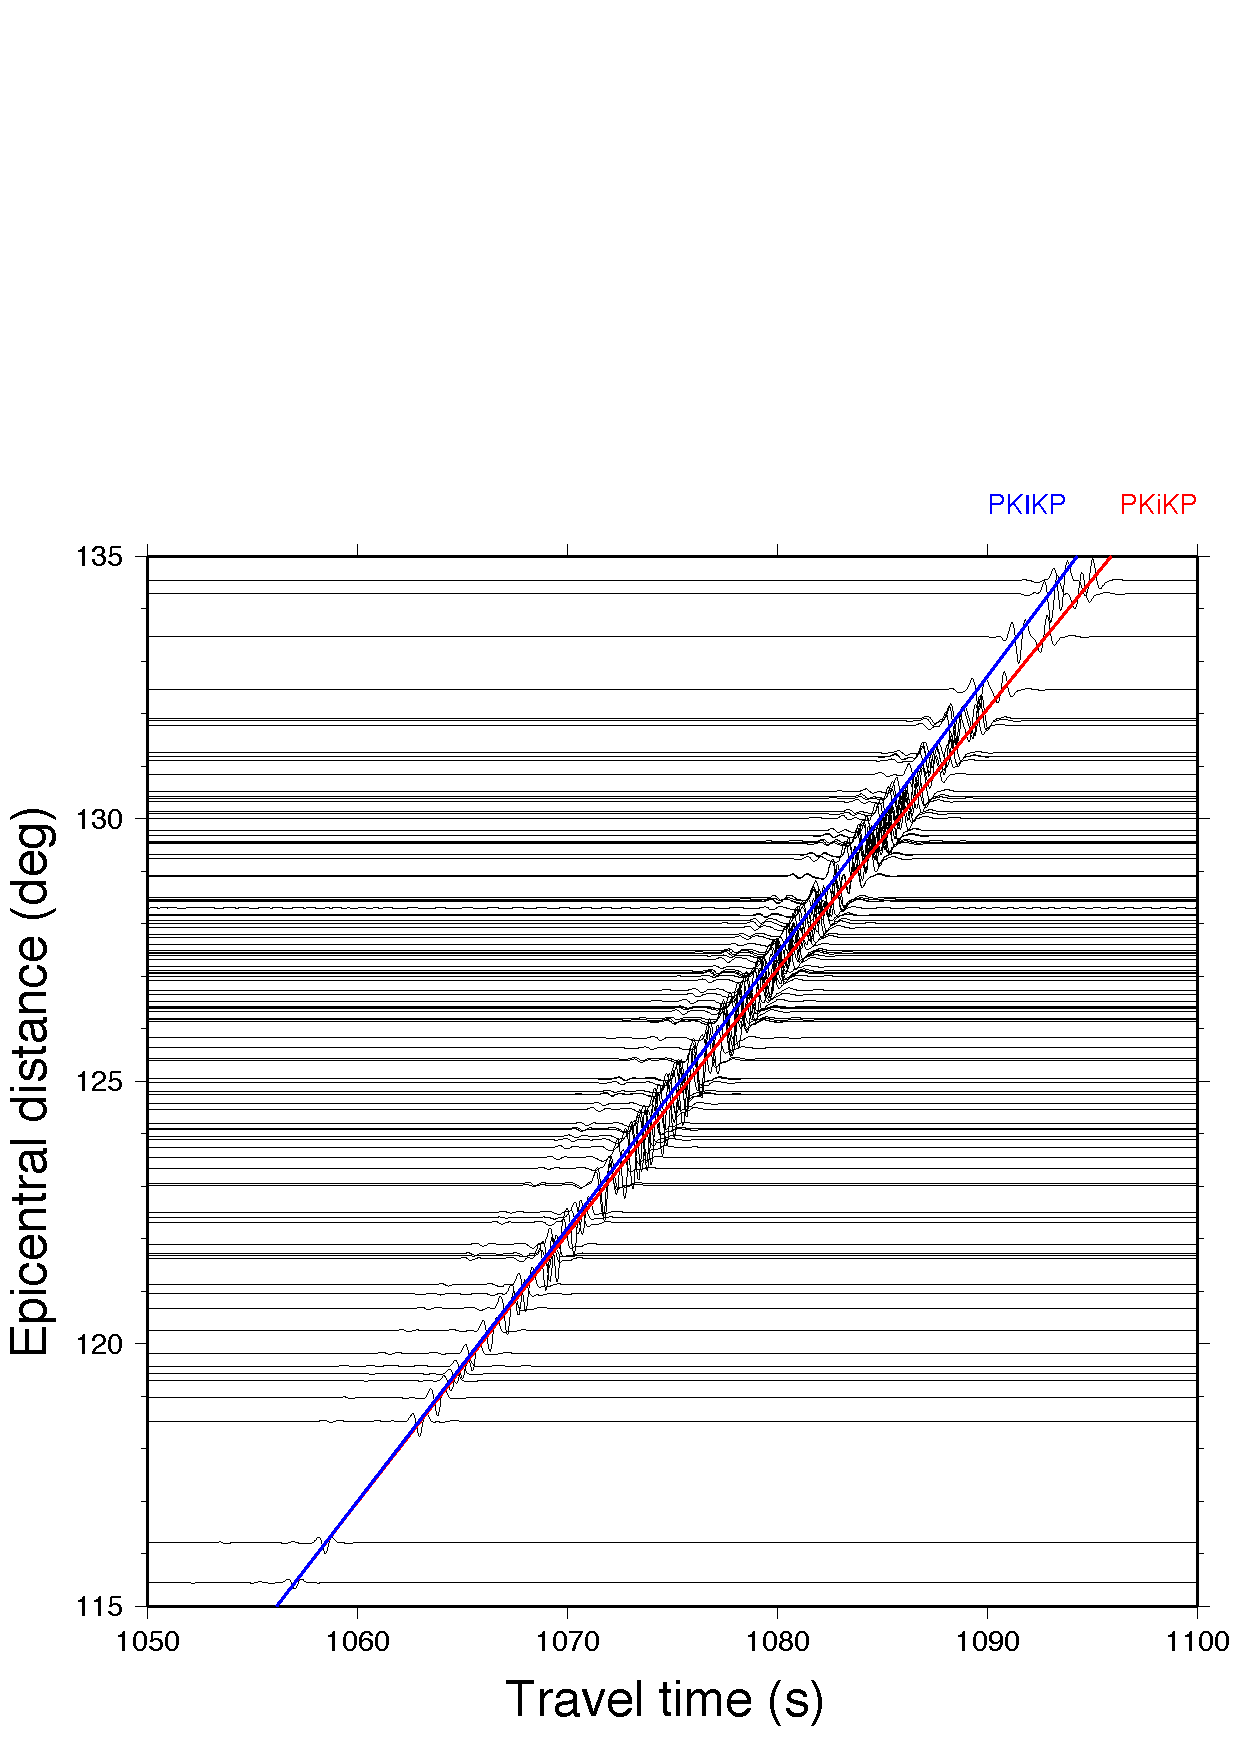
\includegraphics[width=0.6\textwidth]{figures/celebessea/celebessea_synthetic_both.pdf}
	\caption{Real (top) and synthetic (bottom) seismogram data from the Celebes Sea event after event selection. Each seismogram is zeroed on the earthquake time. Over plotted lines are theoretical phase arrivals computed using the AK135 model. Only seismograms with a clear PKIKP arrival are plotted.}
	\label{fig:Real nonaligned}
\end{figure}

In order to more easily visualise the two phases we plot seismograms with individual PKiKP and PKIKP phases. In conjunction we also plot synthetic seismograms with both phases present, called `combined' seismograms from now on. This seismogram simulates the real world where both phases are present.

Each synthetic and real seismogram is shifted such that the initial PKIKP downswing occurs at zero time. This is shown in figure \ref{fig:Synth aligned}. It is now clear to see the PKiKP phase merging with the PKIKP phase at low epicentral distances in the combined seismogram. We are now in a position to take residual measurements on both real and synthetic data. Before we do this, we first take a detour to examine the limits of PKIKP-PKiKP travel time analysis.

\begin{figure}
	\centering
	\includegraphics[width=0.45\textwidth]{figures/bandasea/bandasea_PKIKP_aligned-1}
	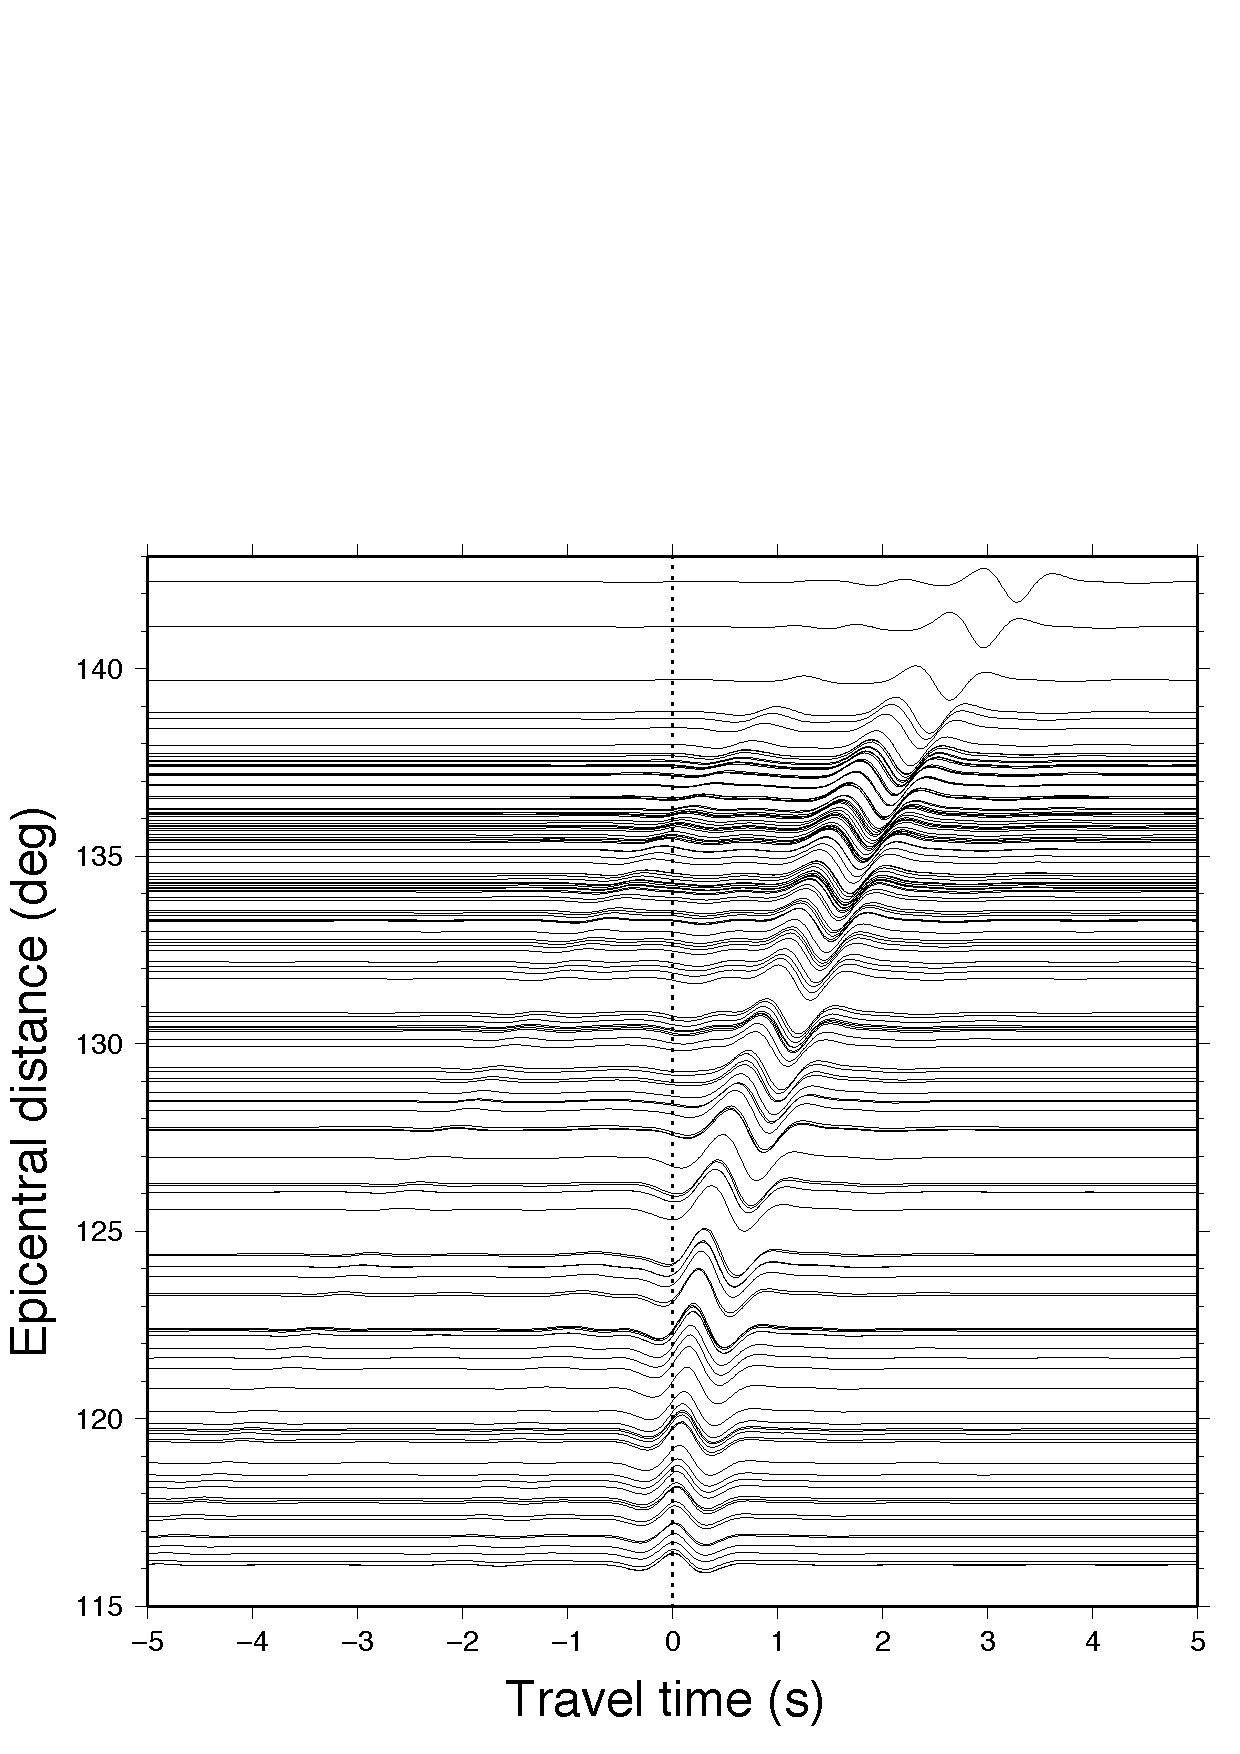
\includegraphics[width=0.45\textwidth]{figures/bandasea/bandasea_PKiKP_aligned}
	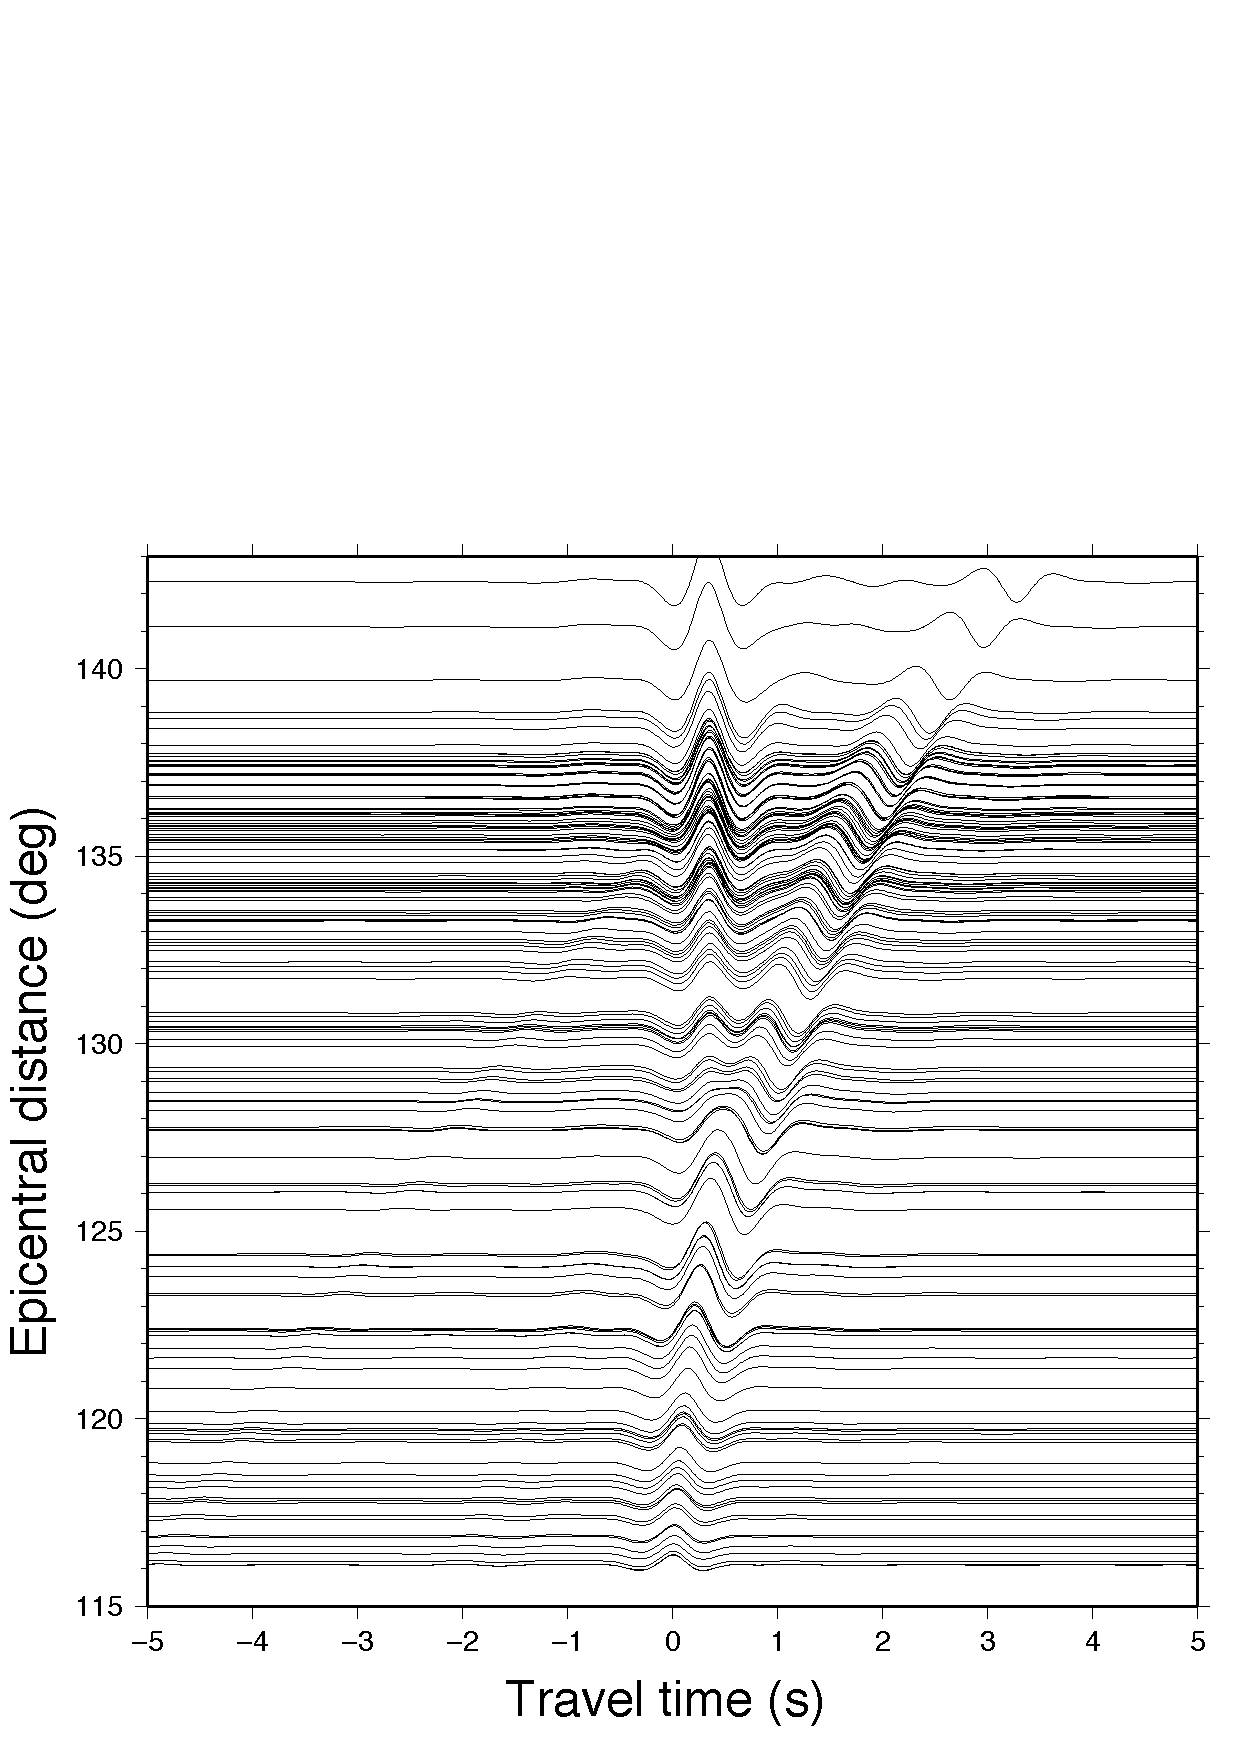
\includegraphics[width=0.45\textwidth]{figures/bandasea/bandasea_both_aligned}
	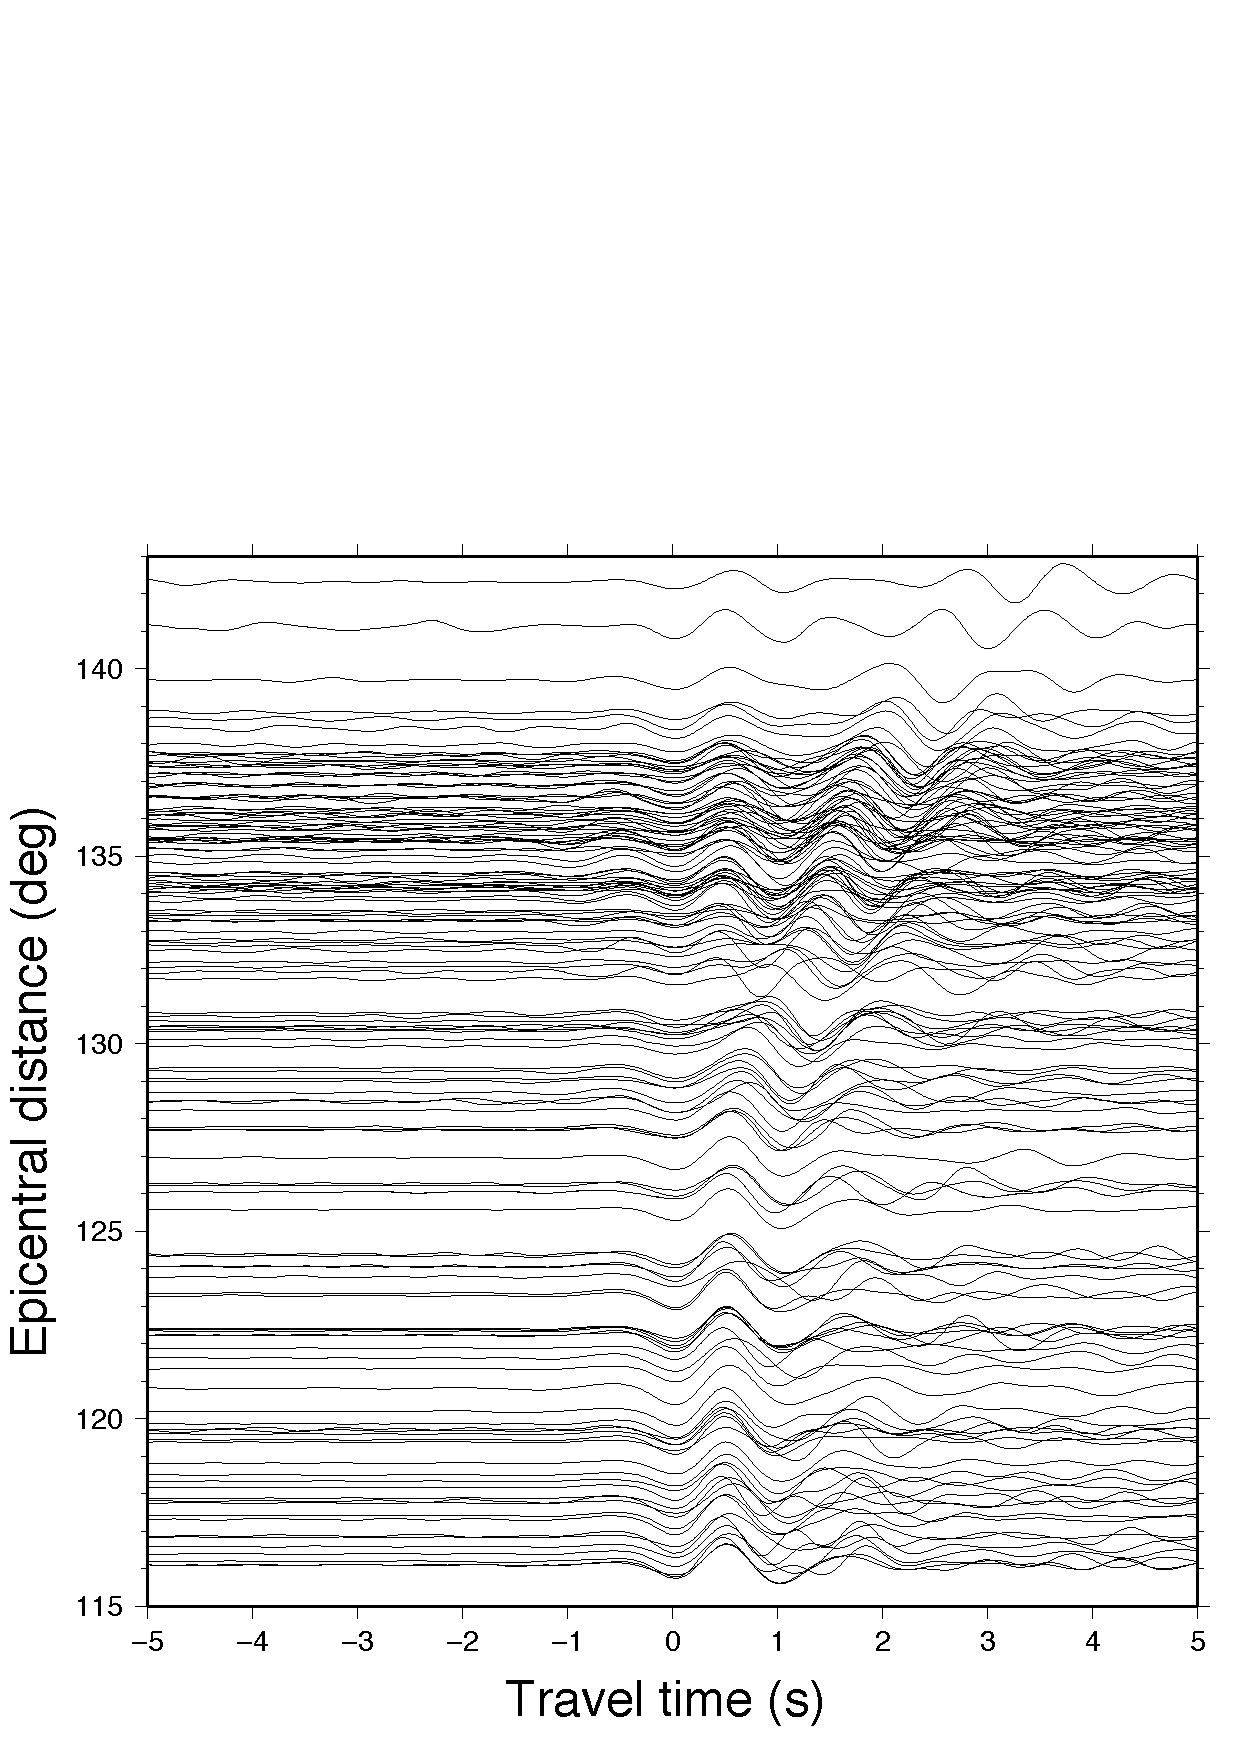
\includegraphics[width=0.45\textwidth]{figures/bandasea/bandasea_real_aligned}
	\caption{Separated PKIKP (top left) PKiKP (top right), combined synthetic (bottom left) and real (bottom right) seismograms for the Banda Sea event. All seismograms are aligned to a common zero time corresponding to the initial PKIKP downswing.}
	\label{fig:Synth aligned}
\end{figure}

%%%%
\section{The limits of PKiKP-PKIKP travel time analysis}
\label{sec:Limits}

In this section we seek to quantitively measure the limits of PKiKP-PKIKP travel time analysis when used to measure the velocity structure at the top of the inner core. Previous studies have only measured up to epicentral distances where PKiKP and PKIKP are clearly distinct phases; in this study we attempt to extend the methodology to much lower epicentral distances. As such it will be useful to know at what distances we can make reliable PKiKP-PKIKP measurements using synthetic data, which acts as a proxy for real world data.

Because we do not know a-priori the actual velocity structure being measured in the real world, we perform synthetic analysis on the three distinct velocity models shown in figure \ref{fig:Velocity models}. Our two new models represent realistic East Hemisphere (EH) and West Hemisphere (WH) isotropic velocity models based on \cite{Waszek2011a}. In each case models are identical to AK135, with the velocity jump at the ICB is modified from 11.0427 km/s to 11.0 km/s (EH) and 11.1 km/s (WH).

\begin{figure}
	\centering
	\includegraphics[width=0.7\textwidth]{figures/velocity_models}
	\caption{Velocity models modified from AK135 (yellow line). Velocity jump at the ICB is varied at 11.1 km/s for a Western Hemisphere (WH) model (red line) and at 11.0 km/s for an Eastern Hemisphere (EH) model (blue line). The models outside the plotted region are identical to AK135.}
	\label{fig:Velocity models}
\end{figure}

\subsection{Minimum resolvable depth}
The only two features that are measurable at all distances in combined synthetic seismograms are the initial downswing and the final downswing (see figure \ref{fig:Synth aligned} bottom left). When making measurements of real data we want to be sure that we are measuring a PKIKP feature (initial downswing) and PKiKP feature (final downswing), and not two PKiKP features. Because the PKiKP amplitude does not decrease with epicentral distance, the right downswing on a combined seismogram is always a PKiKP feature. At lower epicentral distances (and hence depths), due to the PKIKP amplitude decreasing (see figure \ref{fig:Synth aligned}, top left) and PKiKP developing a large downswing to the left (see figure \ref{fig:Synth aligned}, top right), we cannot nescessarily attribute the initial downswing on a combined seismogram to PKIKP. We note that distinguishing the two is not a problem when using synthetic data, where we can take measurements from seismograms that plot only one phase at a time.

To quantify where measurements on the combined seismogram become inaccurate, we plot the difference between PKIKP initial downswings (top left, figure \ref{fig:Synth aligned}) and combined initial downswings (bottom left, figure \ref{fig:Synth aligned}). On the same figure we also plot the difference between PKiKP initial downswings and PKIKP initial downswings. This data is shown in figure \ref{fig:Downswing differences}. A three point moving average is applied in order to smooth the data; this does not significantly change the distribution of data. A depths below 8km PKiKP and combined measurements coincide, showing that in this range the final downswing is actually a PKiKP feature, not a PKIKP feature as we want.

\begin{figure}
	\centering
	\includegraphics[width=0.7\textwidth]{figures/downswing_differences}
	\caption{First downswing measurements for PKiKP and combined synthetic seismograms computed from AK135. Measurements are relative to initial PKIKP first downswings.}
	\label{fig:Downswing differences}
\end{figure}

In figure \ref{fig:Downswing models} we show the same as the combined measurements in figure \ref{fig:Downswing differences}, but for each of our three  velocity models.\footnote{AK135, EH and WH} We find that each curve is similar but offset from the other curves in the depth dimension. Because we do not know the velocity structure we are measuring beforehand, we take deepest point at which the measurements start tailing off to large positive values as a cutoff for depths below which this method cannot be used. This occurs for the WH model (yellow points in figure \ref{fig:Downswing models}) at at a depth of $d_{min} = 10km$.

\subsection{Measuring the average velocity of an uppermost layer}
In the previous section, we showed that there is a certain depth, $d_{min}$, below which we cannot trust PKiKP - PKIKP travel time measurements. This is a function of the average velocity in the layer above $d_{min}$. In this study we take the simplest approach of calculating $d_{min}$ for a range of realistic models, and using the largest value of $d_{min}$ calculated.

However, because the cutoff depth is a function of average velocity in the upper layer, it may be possible to measure this average velocity by measuring $d_{min}$. As we will see later the cutoff is present and measurable in real world data (see figure \ref{fig:Bandasea residuals} and section \ref{sec:Resid measurements}).

For this methdology to be possible the data from an individual event must travel to numerous seismic stations and have a large coverage in the $0km$ - $20km$ depth range. Extensive modelling would also have to be carried out to determine $d_{min}$ as a function of $v_{obs}$. Although not pursued here, we believe this is an investigation that deserves further study\footnote{And could probably occupy another part III student for the best part of a year!}.

\begin{figure}
	\centering
	\includegraphics[width=0.7\textwidth]{figures/downswing_models}
	\caption{Same as blue points in figure \ref{fig:Downswing differences}, but for the three velocity models shown in figure \ref{fig:Velocity models}; AK135 (blue crosses), EH (red crosses), WH (yellow crosses).}
	\label{fig:Downswing models}
\end{figure}

%%%
\subsection{Velocity perturbation calculation errors}
The end goal of this study is to calculate velocity structure perturbations using equation \eqref{eq:Delta v}. The error in an individually measured observed velocity is
\begin{equation}
	\Delta v_{obs} = \Delta \delta v = \frac{v_{model}}{\left( t - \delta t\right )^{2}} t\Delta \delta t 
	\label{eq:Velocity error}
\end{equation}

Table \ref{tab:Error values} gives estimates for the values present in equation \eqref{eq:Velocity error} at a depth of 10km. $t$ is calculated from the AK135 model. $\delta t$ is a worst case estimate based on previous work (\cite{Waszek2011a}). A study perturbing about AK135 could not reduce this value, whereas a study perturbing about a more accurate model could. Finally, measure $\delta t$ two picks are made each on real (synthetic) seismograms which have a sample every 0.2s (0.1s). We attribute an error of 0.1s (0.05s) to one measurement. We also have a systematic error of $0.05s$ caused by the difference in a combined PKiKP measurement and the actual location of the individual PKiKP waveform. This is illustrated at depths below 10km on figure \ref{fig:Downswing models}.

Taking into account these errors we get $\Delta \delta t = 0.17s$. This is a partly a random error which could in theory be reduced arbitrarily close to $0.05s$ by increasing both the synthetic and real sampling rates. It is also reduced by including multiple measurements in a single velocity perturbation calculation.

A value for the worst case error on individual velocity observations in this study\footnote{Corresponding to $\delta t = 1.2s$} is $\Delta v_{obs} = 0.07 km/s$, and the best case error\footnote{Corresponding to $\delta t = -1.2s$} is $\Delta v_{obs} = 0.06 km/s$. This could in theory be reduced to arbitrarily small values be reducing $\Delta \delta t$, as discussed in the previous paragraph.

\begin{table}
\centering
\begin{tabular}{| c | c |}
	\hline
	Parameter		& Estimated value at 10km depth	\\ \hline \hline
	$v_{model}$	& 11.0427 km/s					\\ \hline
	t			& 27.65s						\\ \hline
	$\delta t$		& 1.2s						\\ \hline
	$\Delta \delta t$	& 0.16s						\\				
	\hline
\end{tabular}
\caption{Values used in velocity perturbation error estimation. $\delta t$ is given as a worst case estimate, in order to calculate a worst case error.}
\label{tab:Error values}
\end{table}

%%%%
\section{Residual Measurements}
\label{sec:Resid measurements}

In light of the analysis in the previous section, we now resume where we left off in section \ref{sec:Initial analysis} by making residual measurements. As before we proceed using the Banda Sea earthquake as an example, and present results for all earthquakes at the end.\footnote{See table \ref{tab:Events} for a full event listing and details}

Real seismograms aligned using the same method used for aligning synthetics are shown in the bottom right of figure \ref{fig:Synth aligned}. Peak to peak measurements taken on both the real and synthetic data are shown in figure \ref{fig:Bandasea residuals}. In this figure we plot residual measurements below 10km to illustrate how the real data tapers off, as expected from our analysis on synthetic data in section \ref{sec:Limits}. From now on we only present data take at depths greater than 10km.

\begin{figure}
	\centering
	\includegraphics[width=0.9\textwidth]{figures/bandasea/bandasea_resid}
	\caption{Left hand figure shows individual peak to peak measurements taken for both real data (orange crosses) and synthetic data (blue crosses). Right hand figure shows residuals calculated from the peak to peak measurements.}
	\label{fig:Bandasea residuals}
\end{figure}

Figure \ref{fig:All longitude} shows all measurements as a function of longitude and depth. The vertical line at 15km represents the shallowest depth of previous measurements by \cite{Waszek2011a}. At depths below 15km we see largely positive residuals in the range $10^{\circ}$ to $-170^{\circ}$, and negative residuals in the range $-90^{\circ}$ to $10^{\circ}$. At depths below 15km we see largely positive residuals.

\begin{figure}
	\centering
	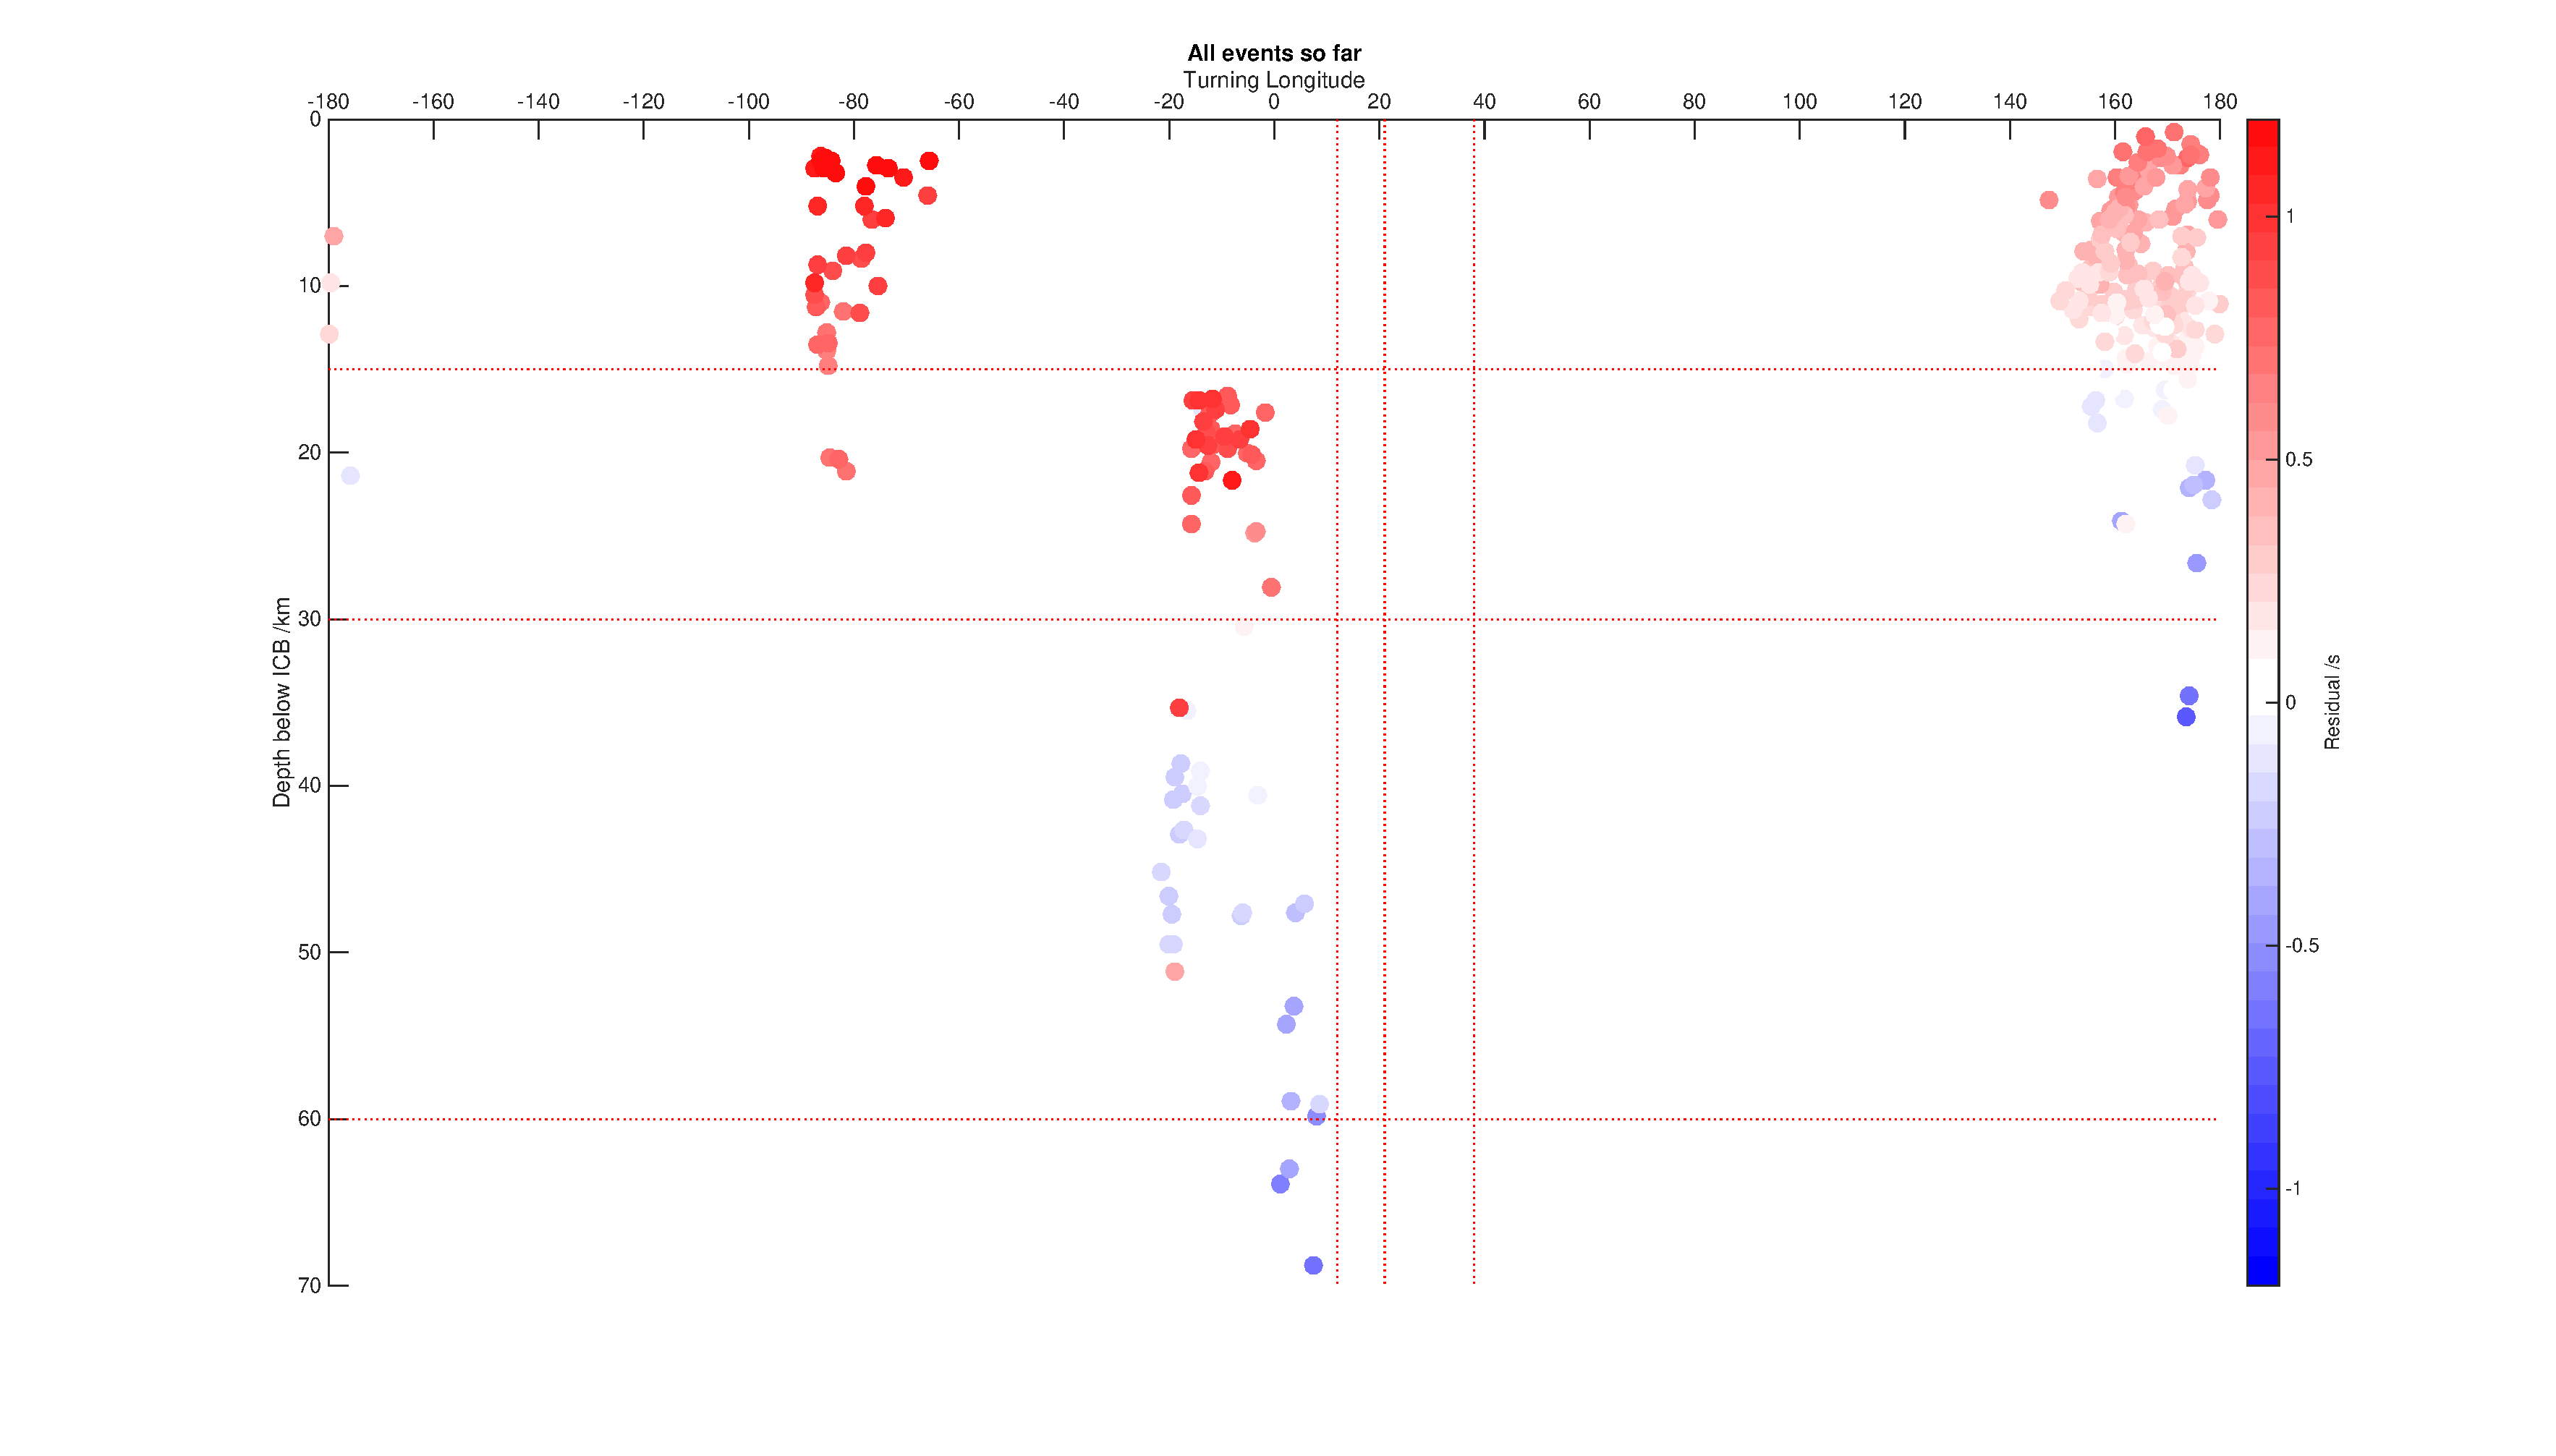
\includegraphics[width=\textwidth]{figures/all_longitude}
	\caption{Measured residuals as a function of turning longitude and bottoming depth below the ICB. Red points indicate positive anomalies, corresponding to rays travelling faster than AK135. Blue points indicate negative anomalies, corresponding to rays travelling slower than AK135. }
	\label{fig:All longitude}
\end{figure}

Figure PUT FIGURE HERE shows measured residuals in the 10km - 15km depth range. We see a clear boundary at $0^{\circ}$; above this longitude there is a lack of measured residuals below 0.1s, whereas below this boundary residuals less than 0.1s are present. This boundary extends the results of \cite{Waszek2011a}, showing that at shallower depths the East Boundary continues to move westward. In the following section we use the $0^{\circ}$ boundary to partition our data for the purposes of calculating regional velocity models.

%%%
\subsection{Velocity models}
To calculate regional velocity models we split our data set up into 4 longitude bins, as indicated on figure \ref{fig:All longitude} and given in table \ref{tab:Velocity models}. In each bin we take individual residual measurements in the range 10km - 15km and calculate velocity perturbations using equation \eqref{eq:Delta v}. In figure \ref{fig:Frac change} we show individual measurements of $v_{obs} / v_{model}$. Negative changes occur in the range [$-110^{\circ}$,$0^{\circ}$] as one would expect from previous research showing a slower western hemisphere. However, the changes are largely positive at all longitudes, indicating a fast layer in the top 10km - 15km of the inner core.

\begin{figure}
	\centering
	\includegraphics[width=\textwidth]{figures/10-15_frac_change}
	\caption{$v_{obs} / v_{model}$ as a function of longitude, calculated from equation \eqref{eq:Delta v}.}
	\label{fig:Frac change}
\end{figure}

To calculate new velocity models, the mean of all the points in a given bin is taken. The error WORK OUT HOW TO WORK OUT THE ERROR

Results of this process are given in table \ref{tab:Velocity models}. All observed velocities are greater than model velocities; we defer discussion on whether this is due to systematic error to PUT SECTION REFERENCE HERE. Variation in observed velocities is consistent with a slower Western Hemisphere and faster Western Hemisphere.

\begin{table}
\centering
\begin{tabular}{| c | c | c | c |}
	\hline
	Longitude Range			& $v_{obs}$ / km/s	& $v_{obs} - v_{model}$ / km/s	& $\delta v_{obs}$ / km/s	\\ \hline \hline
	$150^{\circ}$ - $-170^{\circ}$	& 11.1017			& 0.0508					& 0.006				\\ \hline
	$-90^{\circ}$ - $-75^{\circ}$	& 11.0681			& 0.0254					& 0.013				\\ \hline
	$-30^{\circ}$ - $0^{\circ}$		& 11.0838			& 0.0411					& 0.007				\\ \hline
	$0^{\circ}$ - $60^{\circ}$		& 11.0923			& 0.0496					& 0.016				\\
	\hline
\end{tabular}
\caption{Calculated velocity perturbations for a 10km - 15km depth layer below the ICB. Longitude ranges are indicated on figure \ref{fig:All longitude}. All ranges have $v_{model} = 11.0427 km/s$.}
\label{tab:Velocity models}
\end{table}

%%%%
\section{Discussion and Conclusions}

%%%
\subsection{PKIKP - PKiKP analysis limits}
For the first time the limits of using PKIKP - PKiKP residual measurements to study the velocity structure of the upper inner core has been investigated. Assuming a maximum possible P wave velocity of $11.1 km/s$ in the upper inner core, at depths shallower than $d_{min} = 10km$ below the ICB it is impossible to identify the PKIKP phase in real data. and it is therefore impossible to make individual measurements.

However, we have found that $d_{min}$ is a function of the average velocity in the upper layer of the inner core. Measuring $d_{min}$ is possible on graphs that plot peak to peak distances against depth (eg. figure \ref{fig:Bandasea residuals}). This offers a new and novel method to determine the average velocity structure of the upper inner core.
%%%
\subsection{New residual measurements and velocity models}
Measuring PKIKP - PKiKP residuals in the 10km - 15km depth region was successful, allowing construction of 4 regional velocity models (table \ref{tab:Velocity models}). Each of these velocity models is larger than AK135 to within error, suggesting the presence of a fast layer. Note that this is what would be observed as a result of systematic error due to PKiKP misidentification. We rule this cause out for the following reasons:

\begin{enumerate}
	\item $10km$ has been taken as a conservative cutoff, and occurs only when the average velocity in the upper layer is no lower than $11.1 km/s$ (figure \ref{fig:Downswing models}).
	\item If the cutoff were indeed lower, this would mean a very high velocity in the upper layer. This would change the exact velocity model, but not the fact that they are positive.
	\item The systematic error that would be induced by this method is only of the order $0.05s$ at depths no shallower than $5km$. This is not big enough to explain the largely positive fractional velocity changes.
\end{enumerate}

CAUSE OF FAST LAYER.

Variations within this fast layer still show the variation expected from a slower Western hemisphere and faster Eastern hemisphere. Despite specifically looking in areas where a sharp boundary has been found, there is no evidence for a sharp boundary in our data.

\subsection{Further work}
An obvious line of further work would be gathering more data points in the 10km - 15km depth region. In this study our dataset is comparatively sparse. More data points would be able to test our hypothesis that the 10km - 15km layer has an overall anomalously fast structure compared to AK135.

Recent research, employing a similar methodology but using different seismic phases (\cite{Yee2014}) has shown a region where variations in travel times cannot be accounted for by a simple hemispherical model. A similar study could easily be carried out using the phases used here, in particular using the plethora of data available from earthquakes occurring in the Singapore and Indonesia region.
% Bibliography
\bibliographystyle{agu}
\bibliography{/Users/dstansby/Physics/Papers/library}

\end{document}